\section{Modèle 3-tiers}
En plus du modèle MVC de base, nous avons choisis de suivre un modèle \emph{3 tiers} plus adapté aux sites internet.
Ce modèle permet d'obtenir un site bien structuré et modulaire.

Ce design est composé de 3 couches,
La couche présentation, métier et donnée.

\subsection{La couche Présentation}
Cette couche est le front-end de notre application, elle correspond au code html générer et vue par l'utilisateur, elle touche tout ce qui est navigation dans le site, ergonomie et effet visuel.
Cette couche est donc générer par nos JSP, et fourni a l'utilisateur l'interface visible par son navigateur.
Elle est aussi responsable de fournir des méthodes d'accès au contrôleur afin de pouvoir naviguer sur notre site.
Elle crée des formulaires ou des liens permettant à l'utilisateur d'envoyer des requêtes à notre contrôleur.

\subsection{La couche Métier}
Le couche métier regroupe toute la logique de notre application, c'est ici que nous retrouverons notre MVC2.

Ce dernier consiste à séparer trois 
entités : le Model, la View et le Controller. \\

Le concept de base veut que le Controller se charge des modifications dans le 
Model et d'actualiser la View.
Le rôle du Model n'est que de stocker et de
fournir les procédés de modification de données au Controller. La View est ce que voit les utilisateurs.
Elle affiche l'interface graphique en fonction de ce 
qu'a demandé le Controller et en fonction des données du Model. \\


\subsubsection{Controller}
Dans le cadre des technologies J2EE, il est souhaité que le Controller soit implémenté par une Servlet unique qui sert d'aiguilleur vers les différentes 
pages du site qui sont des View écrites en JSP. Il existe d'autres servlets 
dans notre projet mais qui ne servent seulement à exécuter les requêtes déléguées par le Controller.\\

\subsubsection{Model}
Le Model est représenté par des classes JavaBeans. Une classe JavaBean est une 
classe Java suivant des directives strictes. Il ne doit pas avoir de 
constructeur et ne doit contenir que les attributs et des mutators (les getter et les setter).
Les Javabeans permettent de faciliter l'utilisation de la base de données. \\
Ce module permet la liaison avec la base de donnée en utilisant l'api de la couche donnée, le module est capable de récupérer des information ou en stocker au travers des Java beans

\subsubsection{View}
De manière générale, un navigateur commence par envoyer une requête au 
Controller qui va rediriger l'utilisateur vers la View correspondante et si 
besoin, utiliser le Model pour compléter le contenu de la View qui est renvoyée en guise de réponse au navigateur.\\
C'est ce module qui permet la liaison avec la couche présentation à l'aide des jsp.
Elle génère dynamiquement la page envoyer à l'utilisateur en fonction d'information obtenu par le contrôleur.

\subsection{La couche Donnée}
La couche donnée correspond a tout les données statique, c'est a dire stocker dans une base de donnée la plupart du temps.
Elle est composé de notre base de donnée Derby ainsi que de la classe DBManager fournissant des méthodes d'accès.

Sont rôle est de fournir les données à la couche métier au travers des javabeans.
Elle permet de les peupler lorsque la couche métier demande des donnée et de les stocker lorsque cela est necessaire.

\subsection{Diagramme}
Notre architecture peux être résumé par ce diagramme
\begin{center}
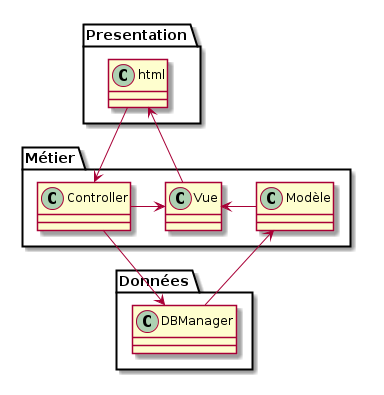
\includegraphics[width=0.6\textwidth]{img/uml}\\
Diagramme des différentes couche et de notre MVC
\end{center}
